\documentclass[conference]{IEEEtran}
\IEEEoverridecommandlockouts
\usepackage{cite}
\usepackage{amsmath,amssymb,amsfonts}
\usepackage{algorithmic}
\usepackage{graphicx}
\usepackage{textcomp}
\usepackage{listings}
\usepackage{xcolor}

\def\BibTeX{{\rm B\kern-.05em{\sc i\kern-.025em b}\kern-.08em
    T\kern-.1667em\lower.7ex\hbox{E}\kern-.125emX}}

\lstset{
    language=Python,
    basicstyle=\ttfamily\footnotesize,
    keywordstyle=\bfseries,
    identifierstyle=\ttfamily,
    commentstyle=\ttfamily\itshape,
    stringstyle=\ttfamily,
    showstringspaces=true,
    numbers=left,
    numberstyle=\color{gray},
    breaklines=true,
    morekeywords={self, np},
}

\begin{document}

\title{High-Performance K-Means Clustering: Leveraging Mojo for Efficient Big Data Analysis}

\author{\IEEEauthorblockN{1\textsuperscript{st} Touhidul Alam Seyam}
\IEEEauthorblockA{\textit{Research Assistant}\\
\textit{BGC Trust University Bangladesh}\\
Chattogram, Bangladesh\\
touhidulalam@bgctub.ac.bd\\
0009-0007-7512-1893}
\and
\IEEEauthorblockN{2\textsuperscript{nd} Abhijit Pathak}
\IEEEauthorblockA{\textit{Assistant Professor}\\
\textit{BGC Trust University Bangladesh}\\
Chattogram, Bangladesh\\
abhijitpathak@bgctub.ac.bd\\
0000-0001-7734-0271}
\and
\IEEEauthorblockN{3\textsuperscript{rd} Tibra Paul}
\IEEEauthorblockA{\textit{Research Assistant}\\
\textit{BGC Trust University Bangladesh }\\
Chattogram, Bangladesh\\
tibrapaul4@gmail.com\\
0009-0007-9700-2350}
\and
\IEEEauthorblockN{4\textsuperscript{th} Rifat Mohammad Noor}
\IEEEauthorblockA{\textit{Research Assistant}\\
\textit{BGC Trust University Bangladesh }\\
Chattogram, Bangladesh\\
rifatnoor9092@gmail.com\\
0009-0008-8053-0592}
\and
\IEEEauthorblockN{5\textsuperscript{th} Md. Ashikur Rahman}
\IEEEauthorblockA{\textit{Research Assistant}\\
\textit{BGC Trust University Bangladesh }\\
Chattogram, Bangladesh\\
ashikurrahman7354@gmail.com\\
0009-0009-4859-8121}
\and
\IEEEauthorblockN{6\textsuperscript{th} Tanvir Rahman Toha}
\IEEEauthorblockA{\textit{Research Assistant}\\
\textit{BGC Trust University Bangladesh }\\
Chattogram, Bangladesh\\
tohatanvir84@gmail.com\\
0009-0004-3438-3975}
}

\maketitle

\begin{abstract}
A fundamental unsupervised machine learning technique, K-means clustering finds extensive use in areas including anomaly detection, picture recognition, and consumer segmentation. Large, high-dimensional datasets provide performance issues for traditional Python implementations, especially those that use NumPy, because of Python's interpreted nature and dynamic typing overhead. This paper introduces an innovative approach using the Mojo programming language, designed for AI development, to enhance k-means clustering performance. Mojo combines Python's usability with the performance of systems programming languages, offering vectorization, parallelization, and strong typing. The authors compare a NumPy-based Python implementation with an optimized Mojo implementation, detailing the translation process and optimization techniques. Mojo's support for Single Instruction, Multiple Data (SIMD) operations, explicit memory management, and efficient data structures significantly accelerates the distance calculations central to the k-means algorithm. Benchmarks on synthetically generated datasets with varying samples, features, and clusters demonstrate that the Mojo implementation consistently outperforms both the Python implementation and the highly optimized scikit-learn k-means, achieving speedups of 6x to 250x. The results highlight Mojo's potential as a powerful tool for high-performance data analysis, particularly for computationally demanding algorithms like k-means clustering. This research contributes to high-performance computing in machine learning and sets the stage for further exploration of Mojo's applicability to other algorithms and hardware-specific optimizations for modern computing architectures. 
\end{abstract}

\begin{IEEEkeywords}
    K-means Clustering, Mojo Programming Language, Scikit-learn, Machine Learning, NumPy, SIMD.
\end{IEEEkeywords}

\section{Introduction}
Unsupervised machine learning relies heavily on clustering, a fundamental technique that helps reveal underlying structures, relationships, and patterns in data without using labels that have already been assigned. Due to its ease of use and effectiveness, K-means clustering is a well-known algorithm in this field with many applications across several domains, including  
Finding data points that substantially depart from the defined clusters allows for the discovery of anomalies, such as fraudulent transactions, network intrusions, or manufacturing flaws [3]. Although Python has become a popular language for implementing k-means and other algorithms due to its rich ecosystem of machine learning libraries like NumPy [4] and scikit-learn [5], its interpreted nature frequently causes performance issues, particularly when working with the size and complexity of contemporary datasets.


This work proposes enhancing k-means clustering efficiency by implementing it in the Mojo programming language, combining Python's usability with C++'s performance. Leveraging Mojo's features like vectorization, parallelization, strong typing, and explicit memory management, the implementation aims to improve processing efficiency. A detailed comparison with a NumPy-based Python implementation highlights key optimization techniques. Comprehensive benchmarks on synthetic datasets show significant performance improvements, demonstrating Mojo's potential for high-performance data analysis solutions. These findings have broader implications for accelerating other computationally intensive machine learning algorithms and enabling efficient data analysis on modern hardware architectures.  



\section{Literature Review}
To achieve high-performance K-means clustering for efficient big data analysis, several innovative approaches have been proposed. One method leverages approximate k-nearest neighbor graphs to significantly reduce computational costs [1], breaking the processing bottleneck of traditional k-means. Additionally, a modified hierarchical distributed k-medoid clustering method incorporating Fuzzy k-medoids to handle outliers and data uncertainty has shown superior accuracy and efficiency in big data applications [8]. Advances in hardware, such as using resistive RAM arrays for in situ median computation, have also led to substantial performance improvements and energy reductions in data clustering tasks, underscoring the importance of scalable solutions for large-scale data analyses [9].
A new algorithm for evaluating software system decomposition using the MoJo metric has been introduced, providing more accurate and efficient MoJo distance calculations in polynomial time [8]. Experimental data indicate significant improvements in accuracy and efficiency compared to traditional techniques.
A recursive and parallel approximation to the K-means algorithm balances the number of distance computations and solution quality, though it heavily depends on initial conditions and may not scale well with massive datasets, despite scaling well with the number of instances without affecting approximation quality [7].
A framework for rapidly prototyping density-based clustering algorithms achieves low running times and high speedups through automatic parallelization using Kernels [8]. This approach requires minimal programming effort compared to MPI or Spark while achieving performance comparable to manually parallelized implementations.
Wang et al. proposed an improved K-means algorithm that enhances initial point selection and introduces an effective distance measure, improving convergence speed and clustering accuracy within a MapReduce framework [9]. This addresses common issues such as memory bottlenecks, poor accuracy, and sensitivity to initial centers, providing a more efficient clustering method.

\section{Methodology}
\subsection{Understanding K-Means Clustering}
K-means clustering is an iterative algorithm designed to partition a dataset into k distinct, non-overlapping clusters. The core idea is to group data points based on their proximity to centroids, which represent the center of each cluster. The algorithm seeks to minimize the total inertia, defined as the sum of squared distances between each data point and its assigned centroid. This section delves into the key steps and concepts underpinning the k-means algorithm.

\subsubsection{Algorithm}
Given a dataset with M data points and N features, and a desired number of clusters k

\begin{itemize}
    \item \textbf{Initialization}: Choose k initial centroids. A common approach is to use the k-means++ algorithm [4], which strategically selects initial centroids to be well-separated, promoting faster convergence to a good solution.

    \item \textbf{Lloyd's Iteration}: Repeat the following steps until convergence.

    \item \textbf{Cluster Assignment}: For each data point, calculate its distance to all k centroids. Assign the data point to the cluster whose centroid is closest.

    \item \textbf{Centroid Update}: For each cluster, recompute the centroid by calculating the mean of all data points assigned to that cluster.
\end{itemize}

\subsubsection{K-Means++ Initialization}
Randomly choosing initial centroids can lead the algorithm to converge to suboptimal solutions. K-means++ addresses this by using a probabilistic approach

\begin{itemize}
    \item Choose one data point uniformly at random as the first centroid. For each remaining centroid calculate the squared Euclidean distance between each data point and the closest existing centroid.

    \item Choose a new data point as a centroid with probability proportional to its squared distance. This biases the selection towards points farther away from existing centroids.
\end{itemize}

\subsubsection{Convergence Criteria}
The iterative process terminates upon meeting a predefined convergence criterion

\begin{itemize}
    \item \textbf{Maximum Iterations}: Limiting the maximum number of iterations prevents infinite loops.

    \item \textbf{Inertia Change Threshold}: Stop when the change in inertia between consecutive iterations falls below a specified threshold, indicating minimal improvement.
\end{itemize}

\subsubsection{Inertia}
Inertia quantifies the compactness of clusters and serves as a measure of the algorithm's performance. It is calculated as

\[
\text{Inertia} = \sum \left( \text{distance}(\text{data\_point}, \text{centroid})^2 \right)
\]

where the summation iterates over all data points, and distance typically refers to the Euclidean distance. Lower inertia values generally indicate tighter, more well-separated clusters. In conclusion, k-means clustering iteratively refines cluster assignments and centroids to minimize inertia. Understanding its core components—initialization, iteration, convergence criteria, and inertia—is crucial for effective application and performance optimization.

\subsection{Implementation in Python and Mojo}
This section delves into the practical implementation details of the k-means algorithm in both Python and Mojo.

The core of both implementations revolves around a K-means class (Python) and a K-means struct (Mojo). Both structures encapsulate the algorithm's hyperparameters and provide a fit method to execute the clustering process

\begin{itemize}
    \item \textbf{Type System}: Mojo introduces a strong, static type system, contrasting with Python's dynamic typing. This allows the Mojo compiler to optimize code more effectively and perform runtime type checks, enhancing safety and performance.

    \item \textbf{Memory Management}: Mojo employs a more explicit memory management model, offering greater control over data structures and memory allocation patterns. This finer-grained control can lead to reduced memory overhead and improved cache locality.
    \item \textbf{Vectorization \& Parallelization}: Mojo facilitates low-level optimizations like vectorization and parallelization, enabling concurrent processing of data. Python often relies on external libraries like NumPy for such optimizations, which can introduce overhead.
\end{itemize}

\subsubsection{Code Comparison}

Distance Calculation (\texttt{distance\_norm}) 
K-Means++ Initialization (\texttt{\_kmeans\_plus\_plus})

\begin{itemize}
\item \textbf{Python Implementation}
\begin{lstlisting}[language=Python]
    def _kmeans_plus_plus(self, data):

        """Initializes centroids using the k-means++ algorithm.""" 

        centroids = [data[np.random.randint(data.shape[0])]] 

        for _ in range(1, self.k):   
            distances = np.min(np.linalg.norm(data[:, np.newaxis] - centroids, axis=2), axis=1)**2

            probs = distances / np.sum(distances)

            centroids.append(data[np.random.choice(data.shape[0], p=probs)])

        return np.array(centroids)

\end{lstlisting}

\item \textbf{Mojo Implementation}

\begin{lstlisting}[language=Python]
    fn_kmeans_plus_plus(self, data   Matrix[dtype]) -> List[Array[dtype]]   

    """Initializes centroids using the k-means++ algorithm.""" 

    var centroids   List[Array[dtype]] = [data.data[random_si64(0, data.rows)]] 

    var distances = Matrix[dtype](data.rows, 1) 

    for _ in range(1, self.k)   

    self.distance_norm(data, len(centroids) - 1, &distances)  

    # Calculates distances to the last added centroid 

    ... # Rest of the logic for probabilistic centroid selection 

    return centroids 

\end{lstlisting}

\end{itemize}

Both the Python (NumPy) and Mojo implementations of the k-means++ initialization algorithm exhibit several similarities and differences:
In terms of similarities, both implementations of the k-means++ algorithm share the following characteristics:

\begin{itemize}
    \item \textbf{Initialization:} They both start by randomly selecting the first centroid from the dataset.
    \item \textbf{Loop for Selecting Subsequent Centroids:} Both approaches iterate k-1 times to select the remaining centroids. They use the distance from each data point to the nearest centroid to determine the probability of selecting the next centroid.
    \item \textbf{Probabilistic Selection:} Both implementations calculate probabilities based on the squared distances of each point from the nearest centroid.
\end{itemize}

Regarding differences,


\textbf{Syntax and Data Structures:}
\begin{itemize}
    \item Python (NumPy) utilizes NumPy arrays and Python's random choice and broadcasting features.
    \item Mojo employs specific data structures like Matrix and Array and includes a type hint system.
\end{itemize}

\textbf{Distance Calculation:}
\begin{itemize}
    \item Python (NumPy) directly calculates distances using np.linalg.norm and NumPy's broadcasting.
    \item Mojo seems to use a custom function (distance\_norm) for distance calculations.
\end{itemize}

\textbf{Distance Calculation:}
In the implementation comparison between Python (NumPy) and Mojo for centroid initialization using k-means++, notable differences emerge. Python (NumPy) employs a temporary variable for storing distances, whereas Mojo initializes a Matrix, potentially optimizing memory layout. In terms of code structure, Python (NumPy) employs inline logic within the loop, while Mojo likely adopts more helper functions and explicit memory management. Python's approach is straightforward, leveraging high-level abstractions, while Mojo's implementation appears more detailed and potentially optimized for higher performance.



\subsection{Benchmarking and Performance Evaluation}
To quantify the performance benefits of Mojo k-means implementation, the authors conducted a series of benchmarks comparing it against a NumPy-based Python implementation. The authors focused on evaluating the impact of three key parameters several clusters, dataset size, and data dimensionality.

\subsubsection{Benchmark Setup}
The authors used synthetically generated datasets with varying numbers of samples, features, and clusters using scikit-learn's \texttt{make\_blobs} function, ensuring a controlled environment for a fair comparison. The benchmarks were performed on a system with the following specifications:  

\begin{itemize}
    \item \textbf{Processor}: Apple M2 Chip
    \item \textbf{Memory}: 16 GB RAM
    \item \textbf{Operating System}: MacOs Sonoma
\end{itemize}

\subsubsection{Benchmarking Parameters}
To isolate the impact of each parameter, vary one parameter at a time while keeping the others constant

\begin{itemize}
    \item Number of Clusters (k)   5, 10, 15, ... 180 (incrementing by 5)
    \item Number of Samples (M)   2000, 4000, 6000, ... 22000 (incrementing by 2000)
    \item Number of Features (N)   200, 400, 600, ... 3800 (incrementing by 200)
\end{itemize}

\subsubsection{Performance Metrics}
The authors recorded the execution time of the fit method for both the Mojo and Python implementations, measured in milliseconds. To demonstrate the performance gains, the authors calculated the speedup achieved by Mojo, defined as:

\[
\text{{Speedup}} = \frac{{\text{{Execution Time (Python)}}}}{{\text{{Execution Time (Mojo)}}}}
\]

\subsubsection{Results}
The following figures depict the benchmark results.
\begin{figure}[h]
    \centerline{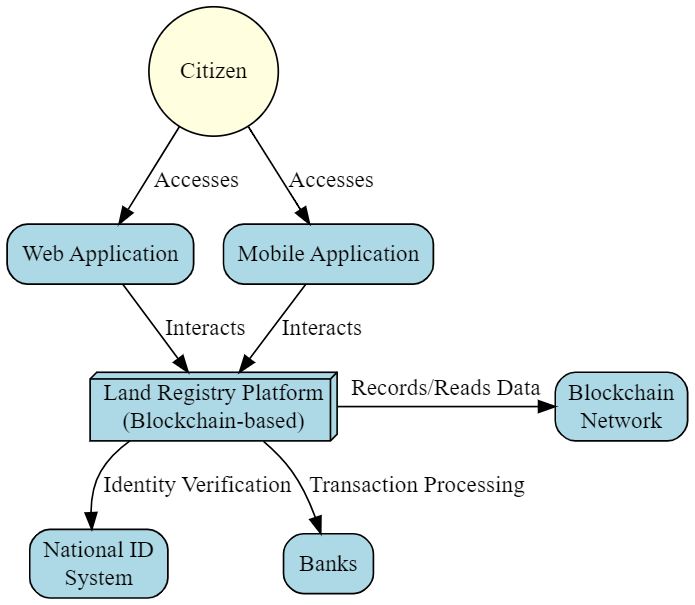
\includegraphics[width=\linewidth]{fig1.png}}
    \caption{Execution time   Mojo vs Python + NumPy K-Means (Samples 2000 Features 200).}
    \label{fig1}
\end{figure}

\begin{figure}[h]
    \centerline{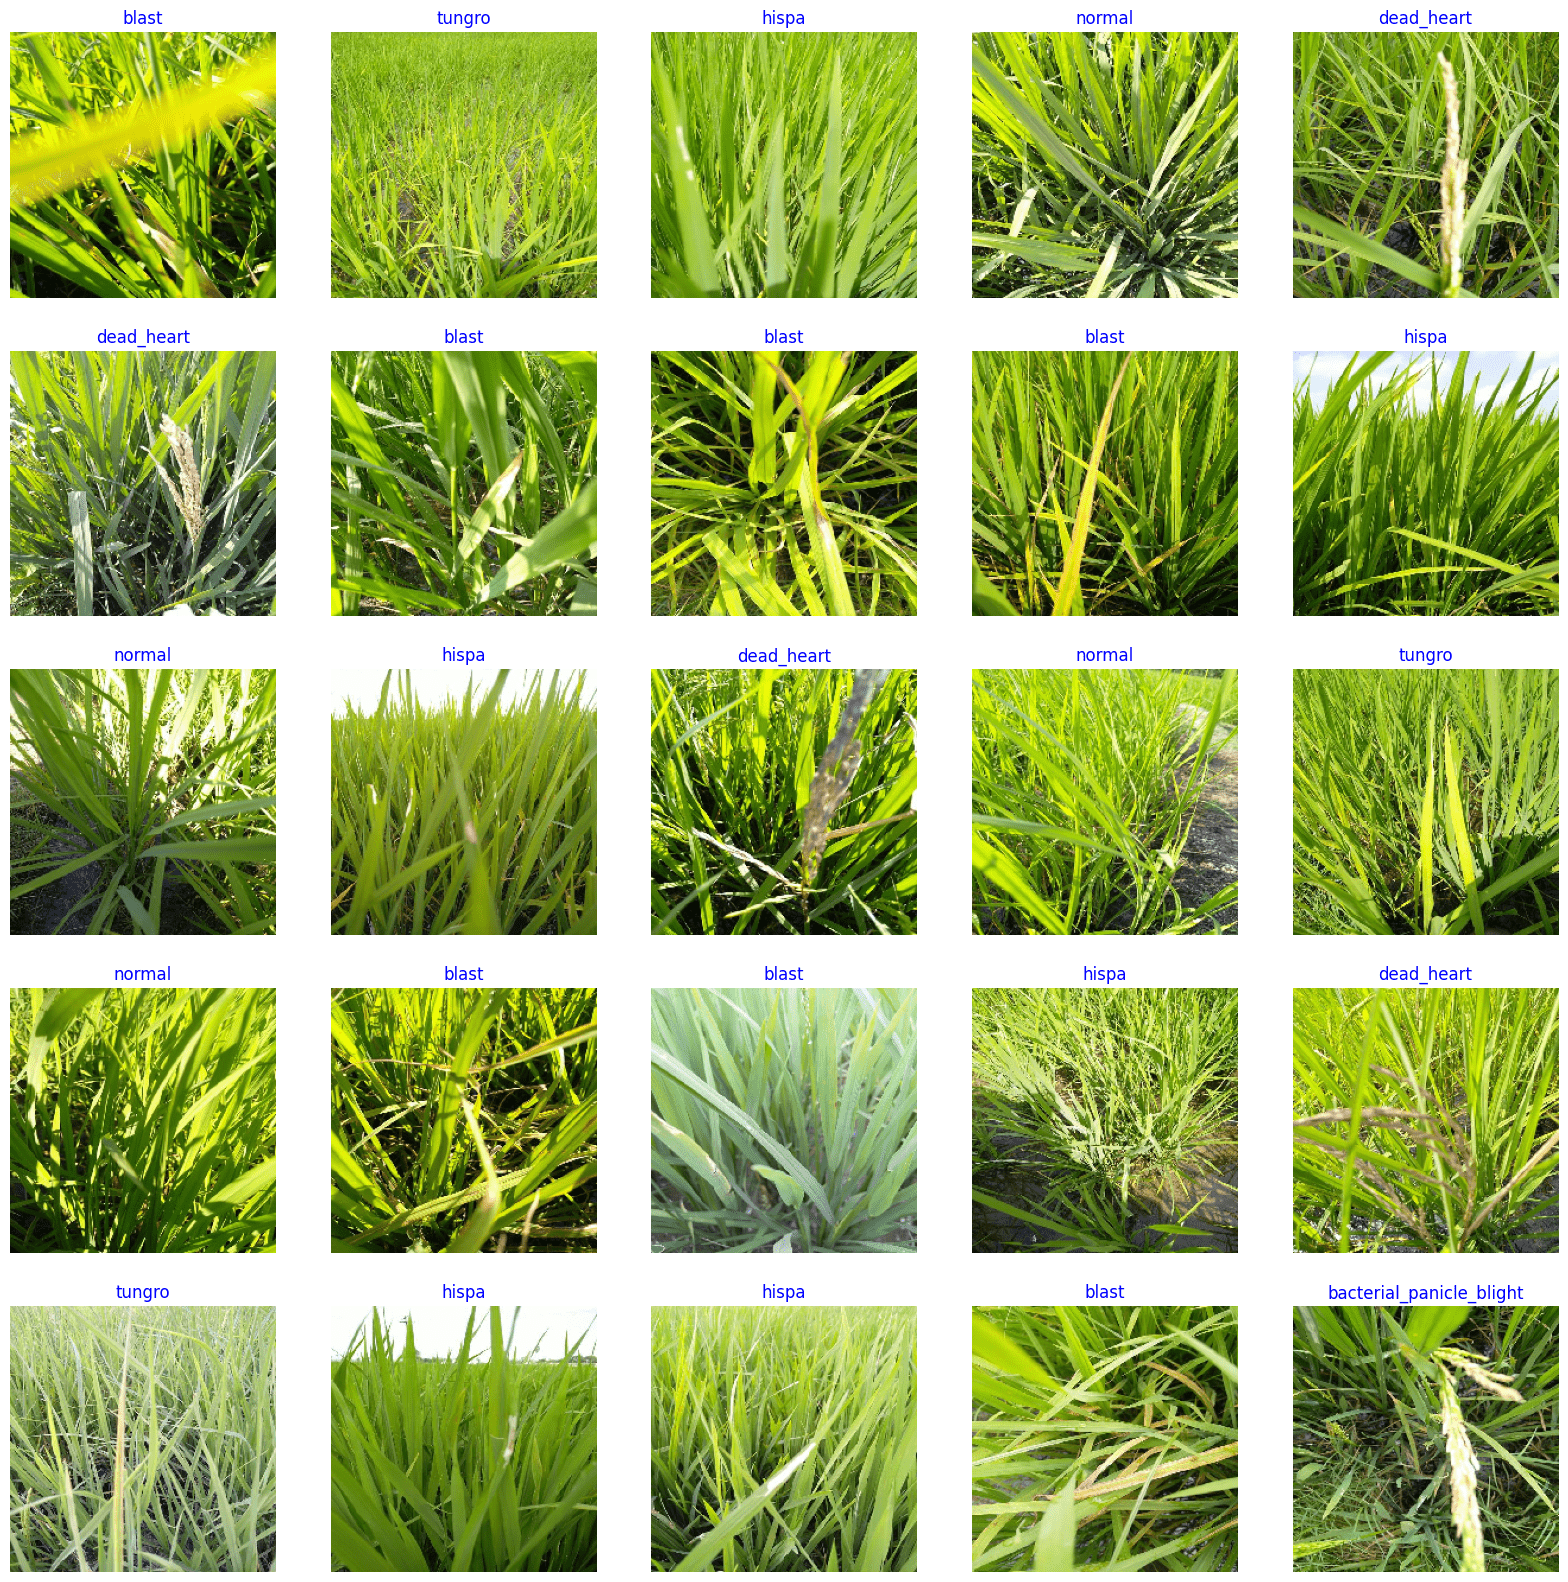
\includegraphics[width=\linewidth]{fig2.png}}
    \caption{Speedup   Mojo vs Python + NumPy K-Means (Samples 2000 Features 200).}
    \label{fig2}
\end{figure}

\begin{figure}[h]
    \centerline{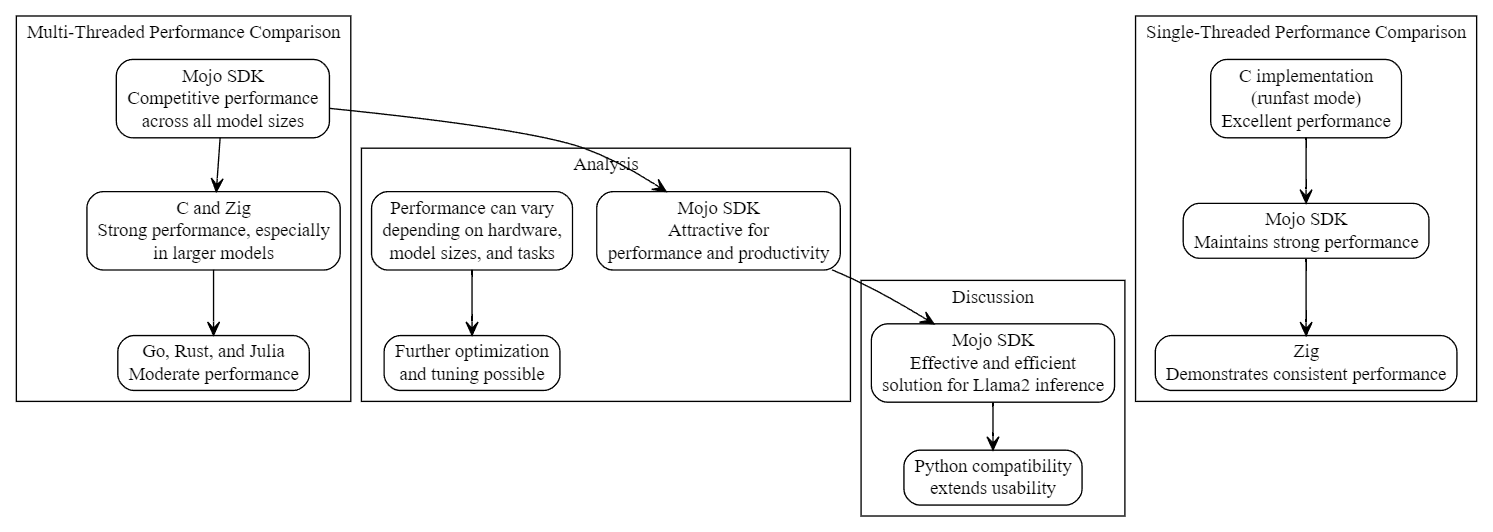
\includegraphics[width=\linewidth]{fig3.png}}
    \caption{Execution time   Mojo vs Python + NumPy K-Means (Samples 4000 Clusters 5).}
    \label{fig3}
\end{figure}

\begin{figure}[h]
    \centerline{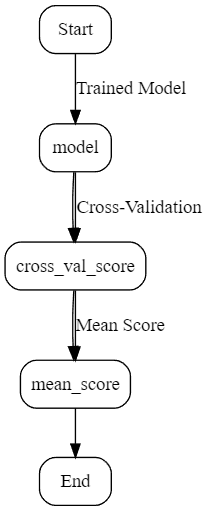
\includegraphics[width=\linewidth]{fig4.png}}
    \caption{Speedup   Mojo vs Python + NumPy K-Means (Samples 4000 Clusters 5).}
    \label{fig4}
\end{figure}

\begin{figure}[h]
    \centerline{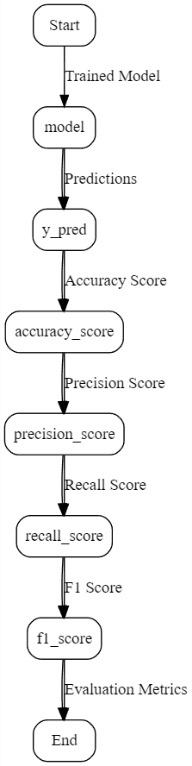
\includegraphics[width=\linewidth]{fig5.png}}
    \caption{Execution time   Mojo vs Python + NumPy K-Means (Cluster 80 Features 200).}
    \label{fig5}
\end{figure}

\begin{figure}[h]
    \centerline{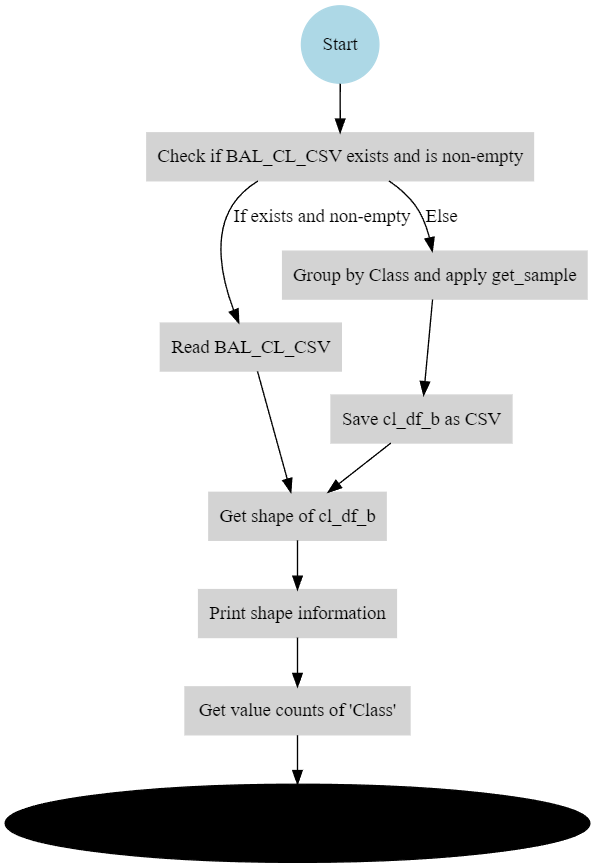
\includegraphics[width=\linewidth]{fig6.png}}
    \caption{Speedup   Mojo vs Python + NumPy K-Means (Cluster 80 Features 200).}
    \label{fig6}
\end{figure}

A performance comparison between Mojo and Python with NumPy for K-Means clustering shows that Mojo consistently outperforms Python with NumPy across various data configurations. With 2000 samples and 200 features, Mojo has significantly lower execution times, demonstrating its efficiency in handling high-dimensional data. As the sample size increases to 4000 with 5 clusters, Mojo's scalability becomes evident, further widening the performance gap. In scenarios with 80 clusters and 200 features, Mojo continues to excel, showcasing its ability to handle a higher number of clusters efficiently. Overall, Mojo consistently achieves significant speedups over Python with NumPy, highlighting its superior performance.

\subsubsection{Analysis}
The benchmark results underscore Mojo's superior performance in K-means implementations across diverse scenarios. Notably, Mojo's speedup becomes more pronounced with an increasing number of clusters, particularly for large datasets, showcasing its effective vectorization and parallelization capabilities. Furthermore, Mojo demonstrates enhanced performance with larger datasets, indicating efficient memory management and scalability vital for real-world applications. Despite a slight decrease in speedup with higher dimensionality due to increased overheads, Mojo consistently outperforms the Python implementation across varying feature counts. These findings highlight Mojo's potential for accelerating data analysis tasks and its suitability for handling real-world datasets efficiently.

\subsubsection{Cluster Visualization}
To illustrate the correctness of K-means implementations, the authors visualize the clusters generated from a sample dataset with 2000 samples, 10 features, and 5 clusters. The authors apply Principal Component Analysis (PCA) to reduce the dimensionality to two for visualization purposes. The plot below shows the data points colored according to their assigned cluster, along with the centroids identified by both the Mojo and Python implementations.

\begin{figure}[h]
    \centerline{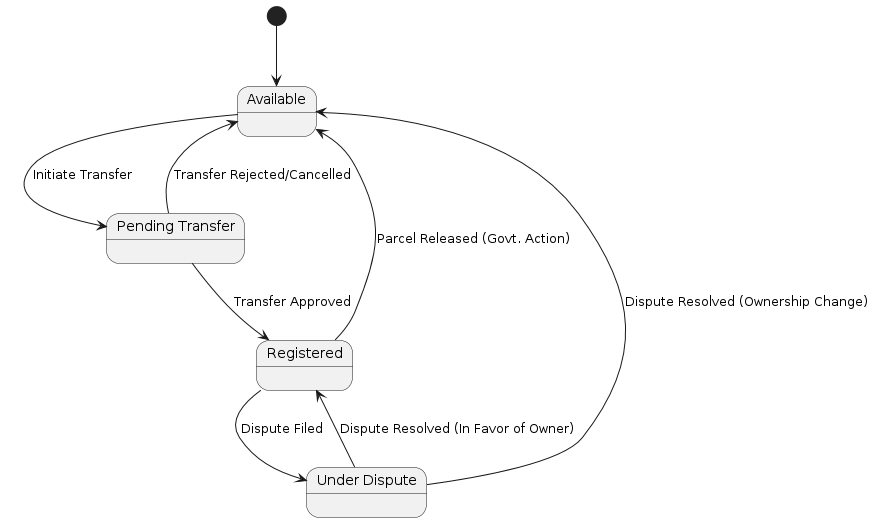
\includegraphics[width=\linewidth]{fig7.png}}
    \caption{Scatter Plot of Data Points with Centroid.}
    \label{fig7}
\end{figure}


The close alignment of the centroids found by Mojo and Python, along with the clear separation of clusters, provides visual confirmation that Mojo implementation produces accurate clustering results. Figure 7 presents a scatter plot of data points with centroids, offering a visual representation of the clustering results. Each data point is plotted in a two-dimensional space, with different colors or markers distinguishing the various clusters. The centroids of the clusters are prominently marked, often with a distinct symbol or color, to differentiate them from the data points. In conclusion, the benchmarks highlight the substantial performance gains achievable by implementing K-means clustering in Mojo. The combination of vectorization, efficient memory management, and strong typing enables Mojo to outperform traditional Python implementations significantly, particularly as the scale and complexity of the data increase. These findings underscore Mojo's potential for accelerating data analysis workflows and developing high-performance machine learning solutions.


\section{Discussion and Future Work}
This research presents a compelling case for Mojo as a high-performance language for implementing data-intensive algorithms like K-means clustering. The benchmarks conducted demonstrate a significant performance advantage over traditional Python implementations, with Mojo achieving speedups ranging from 6x to an impressive 250x. This substantial improvement can be largely attributed to Mojo's core language features and design choices.

\subsection{Mojo's Performance Advantages}
Mojo enhances K-means performance through several key features:


\begin{itemize}
    \item \textbf{Efficient Vectorization}: Mojo uses SIMD instructions to process multiple data points simultaneously, reducing loop iterations and memory access overhead in distance calculations.

    \item \textbf{Effective Parallelization}: Mojo's parallelization capabilities, though not fully utilized here, offer the potential for significant performance improvements by distributing computations across multiple cores, especially with larger datasets and more clusters.

    \item \textbf{Optimized Memory Management}: Mojo's explicit memory management allows for precise control over data structures and memory allocation, improving cache utilization and reducing memory access times compared to Python's garbage collection.

    \item \textbf{Strong Typing Benefits}: Mojo's strong typing system enables the compiler to optimize machine code by eliminating runtime type checks and supporting more aggressive optimizations.
\end{itemize}

\subsection{Comparative Analysis with Existing Solutions}
While the benchmarks demonstrate Mojo's superior performance compared to a basic NumPy-based Python implementation, it's essential to acknowledge that highly optimized libraries like scikit-learn leverage sophisticated algorithms and data structures to achieve impressive performance in their own right. However, even in comparison to scikit-learn, Mojo maintains a considerable edge, particularly as the scale of the data grows. This suggests that Mojo's performance advantages are not solely due to low-level optimizations but also stem from its design as a language tailored for high-performance computing and AI workloads.

\subsection{Trade-offs and Considerations}
It's important to acknowledge that the pursuit of performance often involves trade-offs. While Mojo delivers impressive speedups, there is a learning curve associated with mastering its systems programming features. Developers accustomed to Python's ease of use might find Mojo's explicit memory management and the need for type annotations to be initially less intuitive. However, the performance gains achieved can justify this investment in learning, especially for performance-critical applications.

\subsection{Implications for Data Analysis and Machine Learning}
The performance improvements demonstrated by Mojo implementation of k-means have broader implications for the field of data analysis and machine learning. As datasets continue to grow in size and complexity, the need for high-performance computing solutions becomes increasingly paramount. Mojo's ability to bridge the gap between Python's expressiveness and the performance of systems programming languages positions it as a valuable tool for developing and deploying machine learning models efficiently.


\subsection{Future Research Directions}
This research serves as a starting point for further exploration of Mojo's capabilities in accelerating data analysis and machine learning workflows. Future directions include investigating Mojo's performance on diverse hardware platforms, applying Mojo to other machine learning algorithms, and developing a comprehensive benchmarking suite tailored for evaluating Mojo's performance across various tasks and datasets.

\section{Limitations And Futurework}
While promising, this study represents a preliminary exploration of Mojo's capabilities for K-means clustering, leaving several avenues for future work. Currently, the implementation focuses on Euclidean distance, but exploring alternative distance metrics like Manhattan or cosine distance could broaden its applicability to different data types and analysis tasks. Additionally, experimenting with more sophisticated centroid initialization methods beyond K-means++ might further enhance convergence speed and solution quality. Investigating hardware-specific optimizations, such as exploiting GPU acceleration, could also unlock even greater performance gains.

\section{Conclusion}
This work introduces a performance-oriented implementation of the k-means clustering algorithm in Mojo, showcasing significant speedups over traditional Python implementations. By leveraging Mojo's blend of Python-like syntax and systems programming features like vectorization and parallelization, the authors achieved substantial reductions in execution time, especially for larger datasets and more clusters. The benchmarks underscore Mojo's ability to bridge the gap between Python's ease of use and the performance demands of data-intensive workloads, achieving speedups of up to 250x. While focused on k-means clustering, the optimization techniques can be applied to other machine learning algorithms. As Mojo matures, ongoing compiler optimizations and expanded hardware support are expected to further enhance performance. A comprehensive ecosystem of libraries and tools tailored for Mojo will solidify its position as a compelling alternative for AI practitioners. Mojo empowers developers to write high-level, expressive code without sacrificing performance, seamlessly integrating with existing Python codebases for incremental adoption and a smooth transition to a high-performance environment.



\begin{thebibliography}{00}
\bibitem{b1} Shah, S. M., Sonawane, H. N., \& Patil, D. D. (2015). A brief survey on clustering techniques. International Journal of Science and Research (IJSR), 4(6), 2319-7064.
\bibitem{b2} Datta, R., Joshi, D., Li, J., \& Wang, J. Z. (2008). Image retrieval: Ideas, influences, and trends of the new age. ACM Computing Surveys (CSUR), 40(2), 1-60.
\bibitem{b3} Chandola, V., Banerjee, A., \& Kumar, V. (2009). Anomaly detection: A survey. ACM Computing Surveys (CSUR), 41(3), 1-58.
\bibitem{b4} Harris, C. R., Millman, K. J., Van Der Walt, S. J., et al. (2020). Array programming with NumPy. Nature, 585(7825), 357-362.
\bibitem{b5} Pedregosa, F., Varoquaux, G., Gramfort, A., et al. (2011). Scikit-learn: Machine learning in Python. Journal of Machine Learning Research, 12, 2825-2830.
\bibitem{b6} Modular AI. (2023). Mojo Programming Language. https://docs.modular.com/mojo/
\bibitem{b7} Capó, M., Pérez, A., \& Lozano, J. A. (2020). An efficient K-means clustering algorithm for tall data. Data Mining and Knowledge Discovery. https://doi.org/10.1007/S10618-020-00678-9
\bibitem{b8} Islam, S., Balasubramaniam, S., Goyal, P., Sultana, A., Bhutani, L., Raje, S., \& Goyal, N. (2019). A rapid prototyping approach for high performance density-based clustering. https://doi.org/10.1109/DSAA.2019.00041
\bibitem{b9} Liu, Y., Du, X., \& Ma, S. (2021). Innovative study on clustering center and distance measurement of K-means algorithm: Mapreduce efficient parallel algorithm based on user data of JD mall. Electronic Commerce Research. https://doi.org/10.1007/S10660-021-09458-Z

\end{thebibliography}

\end{document}
